% --------------------------------------------------------------
% This is all preamble stuff that you don't have to worry about.
% Head down to where it says "Start here"
% --------------------------------------------------------------
 
\documentclass[11pt]{article}
 
\usepackage[margin=1in]{geometry} 
\usepackage{amsmath,amsthm,amssymb,amsfonts}
\usepackage{tikz}
   \usetikzlibrary{calc,positioning}
   \tikzset{>=latex}
\usepackage{pgfplots}
\usepackage{bm}
\usepackage{xcolor}
\usepackage{units}
\usepackage{floatrow}
\usepackage{times}
\usepackage{epsfig}
\usepackage{graphicx}
\usepackage{subcaption}
\usepackage[nomarkers]{endfloat}
% \usepackage[numbered, framed]{mcode}
 
\newcommand{\N}{\mathbb{N}}
\newcommand{\Z}{\mathbb{Z}}
\newcommand{\R}{\mathbb{R}}
\newcommand{\X}{\mathcal{X}}
\newcommand{\Xf}{\mathcal{X}_f}
 
\newenvironment{theorem}[2][Theorem]{\begin{trivlist}
\item[\hskip \labelsep {\bfseries #1}\hskip \labelsep {\bfseries #2.}]}{\end{trivlist}}
\newenvironment{lemma}[2][Lemma]{\begin{trivlist}
\item[\hskip \labelsep {\bfseries #1}\hskip \labelsep {\bfseries #2.}]}{\end{trivlist}}
\newenvironment{exercise}[2][Exercise]{\begin{trivlist}
\item[\hskip \labelsep {\bfseries #1}\hskip \labelsep {\bfseries #2.}]}{\end{trivlist}}
\newenvironment{reflection}[2][Reflection]{\begin{trivlist}
\item[\hskip \labelsep {\bfseries #1}\hskip \labelsep {\bfseries #2.}]}{\end{trivlist}}
\newenvironment{proposition}[2][Proposition]{\begin{trivlist}
\item[\hskip \labelsep {\bfseries #1}\hskip \labelsep {\bfseries #2.}]}{\end{trivlist}}
\newenvironment{corollary}[2][Corollary]{\begin{trivlist}
\item[\hskip \labelsep {\bfseries #1}\hskip \labelsep {\bfseries #2.}]}{\end{trivlist}}
 
\begin{document}
 
% --------------------------------------------------------------
%                         Start here
% --------------------------------------------------------------
 
%\renewcommand{\qedsymbol}{\filledbox}
 
\title{Model Predictive Control\\
    Programming Exercise - Report} %replace X with the appropriate number
\author{Gian Andrea M{\"u}ller (14-935-035)\\
    Kevin Anschau Schwarzer (12-914-735)\\
    Ueli Eugen Wechsler (11-920-444)} %replace with your name
%if necessary, replace with your course title

\maketitle

\begin{enumerate}
    % 1.
    \item Interpretation of the matrices $A_c$ and $B_c$:
    
    \begin{enumerate}
    \item
    Rows \textbf{1-3} and \textbf{7-9} of $A_c$ describe how the position / the angle change depending on their respective velocities.
        
    \item Rows \textbf{4} and \textbf{5} of $A_c$ describe the change of the velocity in x- and y-direction depending on gravitational acceleration.
    
    \begin{align}
    \ddot{x}&=9.81\cdot\beta \label{ddotx} \\
    \ddot{y}&=-9.81\cdot\alpha \label{ddoty} \\
    \ddot{z}&=u_1+u_2+u_3+u_4 \label{ddotz}
    \end{align}
    
	Non-zero pitch- and roll-angles result in a non-zero projection of the gravitational acceleration on the body-fixed x- and y-axis. This projection is represented by equations (\ref{ddotx},\ref{ddoty}).
	
Since the system is linearized in $(x_s,u_s)$ such that the effect of gravity is compensated for entirely, $\dot{z}$ is unaffected by gravity even with non-zero roll- and pitch angles.
	\item 
	The sixth row of $B_c$ refers to acceleration of the craft in z-direction depending on the combined thrust of all 4 rotors. (\ref{ddotz})
	\item Row \textbf{10-11} describe how the imbalance between opposing rotors results in an angular acceleration in $\alpha$ and $\beta$. (\ref{ddotalpha},\ref{ddotbeta})
	
	\begin{alignat}{6}
	\ddot{\alpha}=& & 0.56\cdot u_2 &\null &-0.56\cdot u_4 \label{ddotalpha} \\
	\ddot{\beta} = & -0.56\cdot u_1 &&+0.56\cdot u_3 &\label{ddotbeta} \\
	\ddot{\gamma}= & 0.73\cdot u_1&-0.73\cdot u_2&+0.73\cdot u_3&-0.73\cdot u_4 \label{ddotgamma}
	\end{alignat}
	
	\item The last row accounts for the fact that the two rotor pairs turn in different directions and therefore induce a rotation about the z-axis as soon as their respective torques do not add up to zero. (\ref{ddotgamma})
    \end{enumerate}
% subsection nonlinear_model_and_linearization (end)
\end{enumerate}

\newpage
\subsection*{First MPC controller} % (fold)
\label{sub:first_mpc_controller}

\begin{enumerate}
    \setcounter{enumi}{1}
    % 2.
    \item Choice of tuning parameters $(Q,R,P,A_{\Xf},b_{\Xf})$
    
    \begin{align}
    Q &= \text{diag}(10000,\ 4000,\ 9000,\ 5,\ 250,\ 200,\ 1)\\
    R &= 0.1*\text{eye(4)}
    \end{align}

	Reasoning for the chosen Q and R matrices:    
    \begin{itemize}
    \item \textbf{Cheap Control}: Select R to be significantly smaller than Q in order to allow aggressive control action.
    \item \textbf{Prioritize Q}: Chose the respective weights of $\dot{z}$, $\alpha$ and $\beta$ in Q dramatically larger in order to reduce their errors fast. The asymmetry in $\alpha$ and $\beta$ compensates for the different convergence of the two and results in a relatively symmetric reaction for all following applications.
    
    \vspace{2ex}
    
    In addition, to help with the reduction of errors in $\alpha$ and $\beta$ the weights of $\dot{\alpha}$ and $\dot{\beta}$ are increased slightly.
    
    \vspace{2ex}
    
    Finally the weight of $\gamma$ is chosen relatively low since only a slow regulation is required there.
    \end{itemize}
    
    \begin{equation}
    P=\begin{bmatrix}1&0&0&0&0&0&0\\0&1.419&0&0&0.056&0&0&\\0&0&2.291&0&0&0.077&0\\0&0&0&0.0034&0&0&0\\0&0.056&0&0&0.0296&0&0\\0&0&0.077&0&0&0.0258&0\\0&0&0&0&0&0&0.0004\end{bmatrix}
    \end{equation}
    
    The P-matrix shown above results from the implementation of an LQR-controller based on the system model as well as Q and R.
    
    \begin{verbatim}
    [K_inf,P_inf,~] = dlqr(sys.A,sys.B,Q,R);
    \end{verbatim}
    
    Consequently we apply the resulting control-law to get a closed loop system. After imposing state- and input constraints we are ultimately able to calculate the final set which in this case is the \textbf{LQR maximum control invariant set}.

    % 3.
    \item The response of the first MPC controller can be seen in
    Figure~\ref{fig:1st_mpc_controller}.
    \begin{figure}[ht]
        \centering
        \begin{subfigure}[c]{0.3\linewidth}
            \centering
            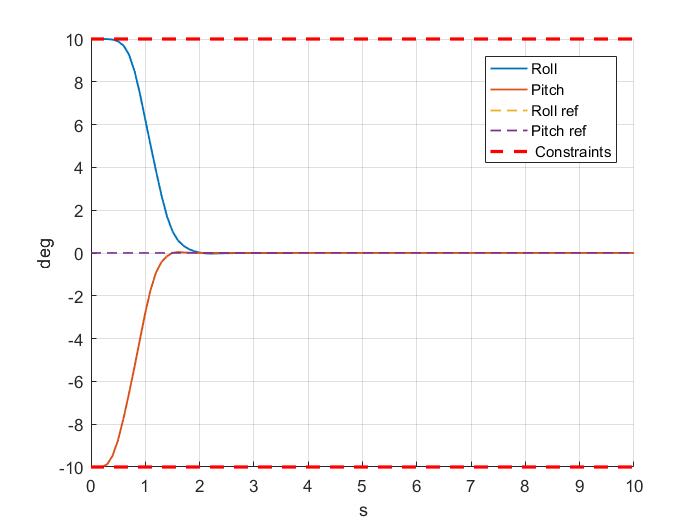
\includegraphics[width=\linewidth]{Plots_03_FirstMPCController/01}
            \caption{Roll- and Pitch}
        \end{subfigure}
        ~
        \begin{subfigure}[c]{0.3\linewidth}
            \centering
            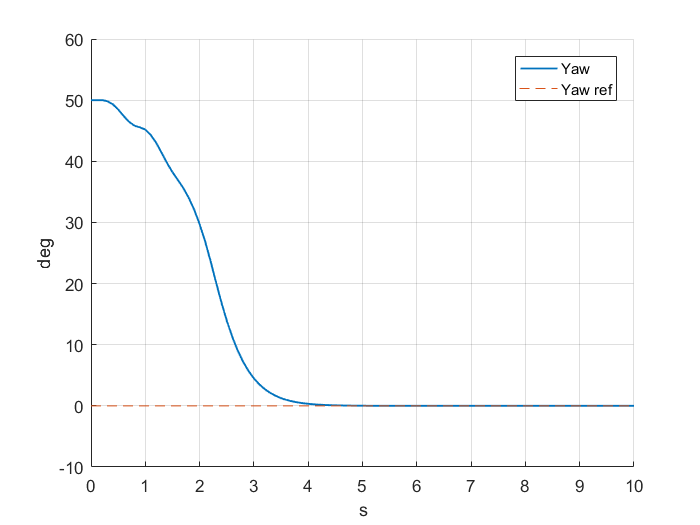
\includegraphics[width=\linewidth]{Plots_03_FirstMPCController/02}
            \caption{Yaw}
        \end{subfigure}
        ~
        \begin{subfigure}[c]{0.3\linewidth}
            \centering
            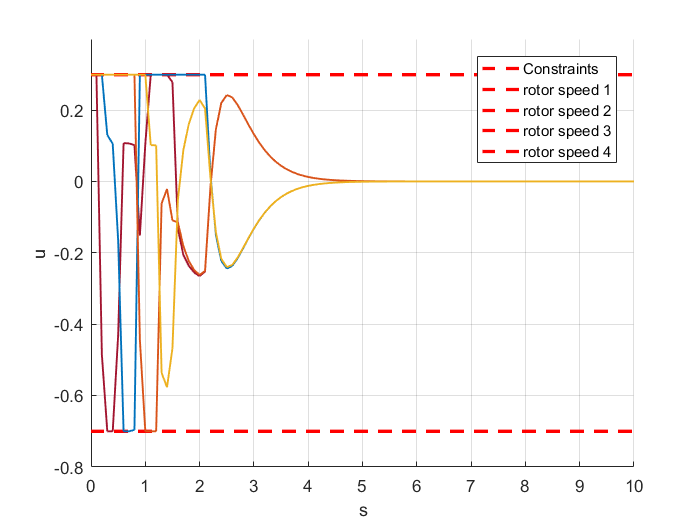
\includegraphics[width=\linewidth]{Plots_03_FirstMPCController/03}
            \caption{Rotor Speeds}
        \end{subfigure}

        \begin{subfigure}[c]{0.3\linewidth}
            \centering
            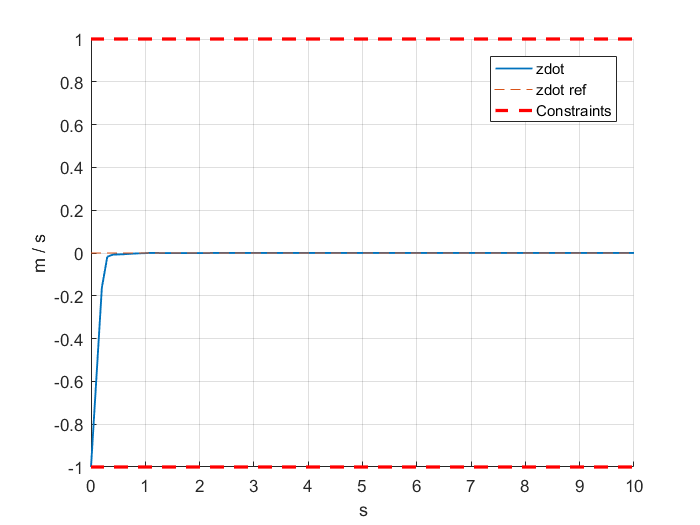
\includegraphics[width=\linewidth]{Plots_03_FirstMPCController/04}
            \caption{zdot}
        \end{subfigure}
        ~
        \begin{subfigure}[c]{0.3\linewidth}
            \centering
            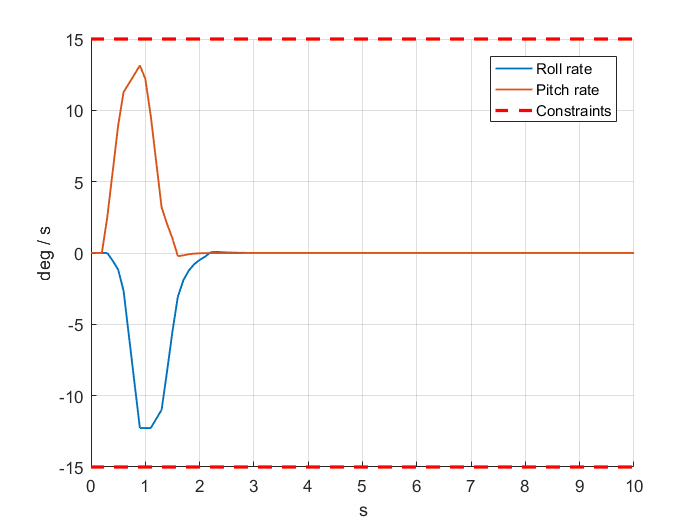
\includegraphics[width=\linewidth]{Plots_03_FirstMPCController/05}
            \caption{Roll and Pitch rates}
        \end{subfigure}
        ~
        \begin{subfigure}[c]{0.3\linewidth}
            \centering
            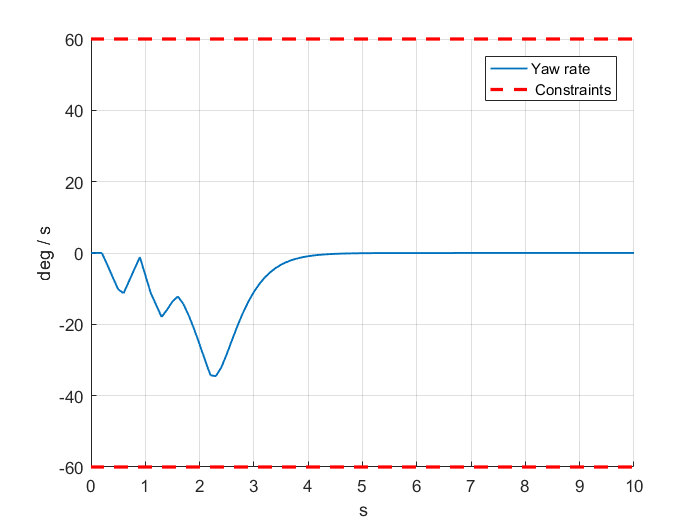
\includegraphics[width=\linewidth]{Plots_03_FirstMPCController/06}
            \caption{Yaw rate}
        \end{subfigure}
        \caption{Response of first MPC controller.}
        \label{fig:1st_mpc_controller}
\end{figure}
\end{enumerate}

% subsection first_mpc_controller (end)


\newpage
\subsection*{Reference Tracking} % (fold)
\label{sub:reference_tracking}

\begin{enumerate}
    \setcounter{enumi}{3}
    % 4.
    \item Define the state $(x_r,u_r)$ as a function of an arbitrary reference.
    
    To find the target state $(x_r,u_r)$ we remind ourselves that we want to find some desirable state $x_r$ and a corresponding input signal $u_r$ which result in a steady state of the system and produce an output $y=r$. Formulated mathematically this results in the following system of equations.
    
    \begin{align}
    \underbrace{\begin{bmatrix}I-A&-B\\C&0\end{bmatrix}}_{\text{LHS}}\begin{bmatrix}x_r\\u_r\end{bmatrix}&=\begin{bmatrix}0\\r\end{bmatrix}\\
    \end{align}
    
    To solve the system above the matrix on the left hand side is inverted and multiplied with the right hand side. In matlab this works as follows:
    
    \begin{verbatim}
    TargetState = LHS\[zeros(nx,1); ref];
    xr = TargetState(1:nx);
    ur = TargetState(nx+1:end);
    \end{verbatim}
    
    Herein the sdpvariable \verb|ref| is used to make the calculation depend on any reference signal handed over later by simQuad.

    % 5.
    \item The response for the constant reference signal can be seen in
    Figure~\ref{fig:constant_reference_with_offset}.
    \begin{figure}[ht]
        \centering
        \begin{subfigure}[c]{0.3\linewidth}
            \centering
            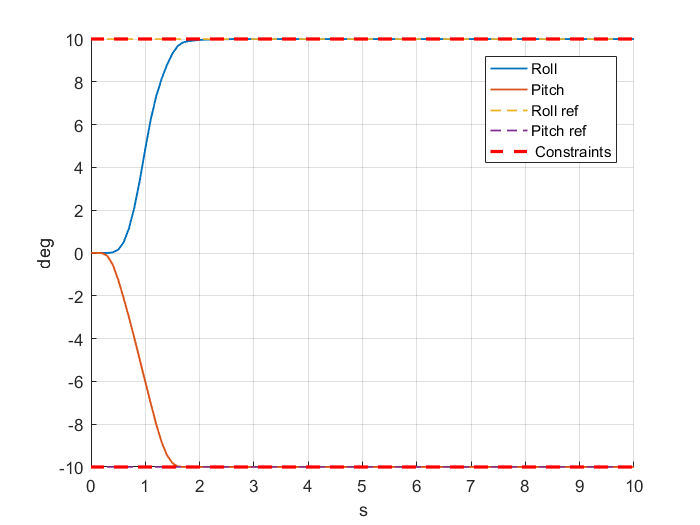
\includegraphics[width=\linewidth]{Plots_05_ReferenceTracking_Constant/01}
            \caption{Roll and Pitch}
        \end{subfigure}
        ~
        \begin{subfigure}[c]{0.3\linewidth}
            \centering
            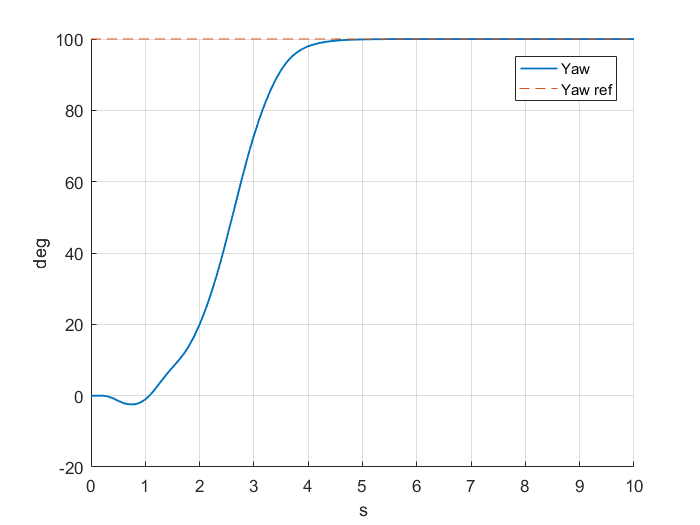
\includegraphics[width=\linewidth]{Plots_05_ReferenceTracking_Constant/02}
            \caption{Yaw}
        \end{subfigure}
        ~
        \begin{subfigure}[c]{0.3\linewidth}
            \centering
            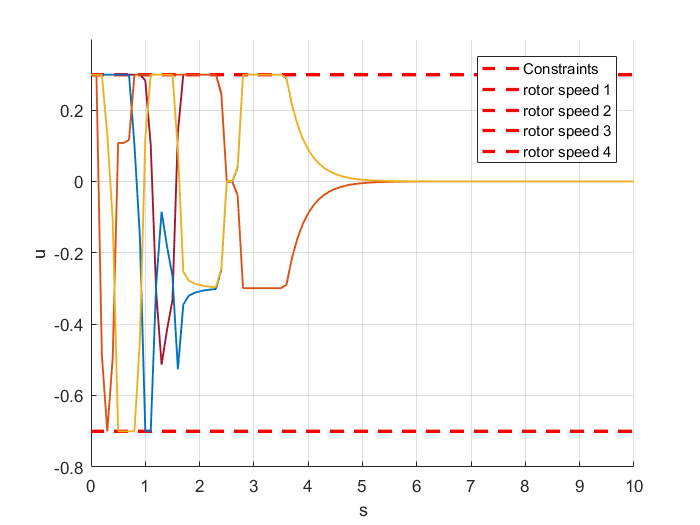
\includegraphics[width=\linewidth]{Plots_05_ReferenceTracking_Constant/03}
            \caption{Rotor Speeds}
        \end{subfigure}

        \begin{subfigure}[c]{0.3\linewidth}
            \centering
            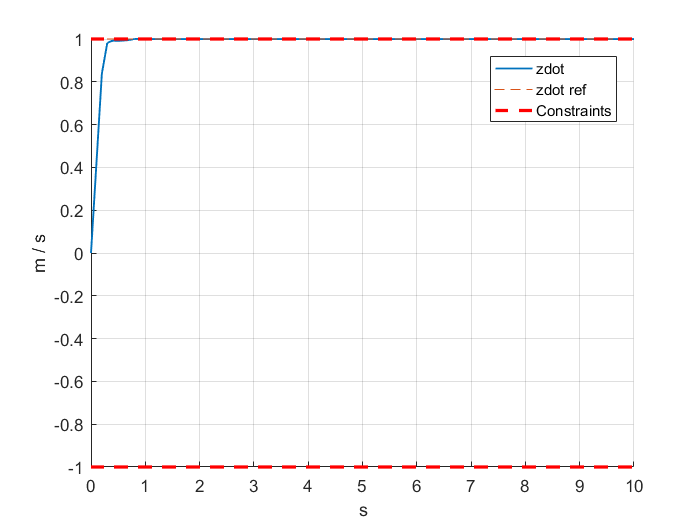
\includegraphics[width=\linewidth]{Plots_05_ReferenceTracking_Constant/04}
            \caption{zdot}
        \end{subfigure}
        ~
        \begin{subfigure}[c]{0.3\linewidth}
            \centering
            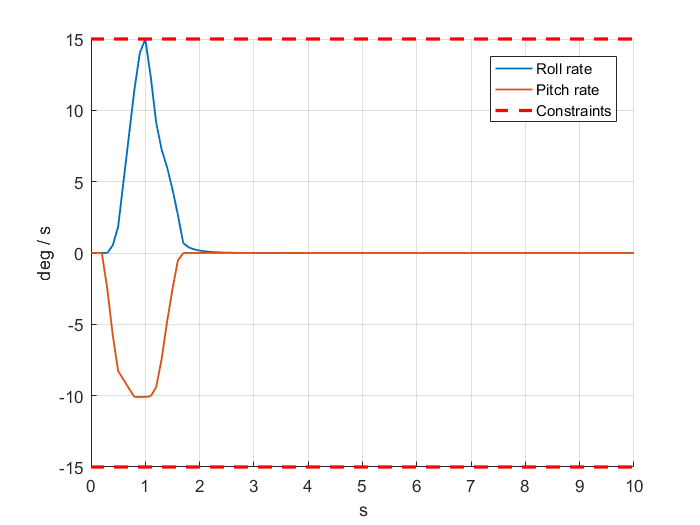
\includegraphics[width=\linewidth]{Plots_05_ReferenceTracking_Constant/05}
            \caption{Roll and Pitch rates}
        \end{subfigure}
        ~
        \begin{subfigure}[c]{0.3\linewidth}
            \centering
            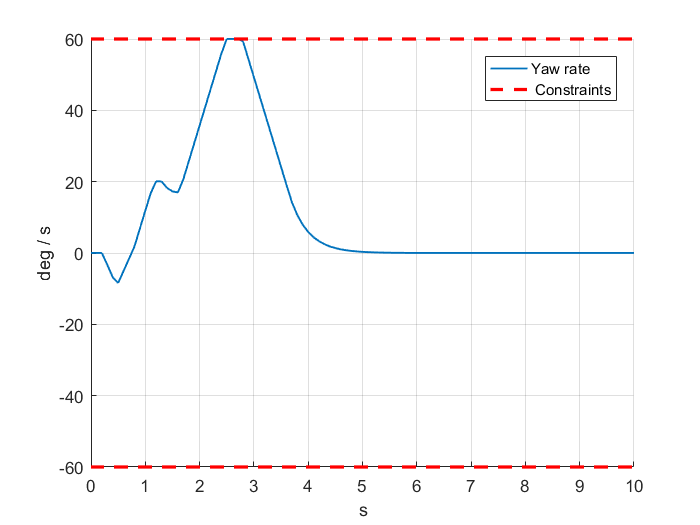
\includegraphics[width=\linewidth]{Plots_05_ReferenceTracking_Constant/06}
            \caption{Yaw rate}
        \end{subfigure}
        \caption{Response for constant reference signal with offset.}
        \label{fig:constant_reference_with_offset}
\end{figure}

    % 6.
    \item The response for the slowly varying reference signal can be seen in
    Figure~\ref{fig:varying_reference_with_offset}.
    \begin{figure}[ht]
        \centering
        \begin{subfigure}[c]{0.3\linewidth}
            \centering
            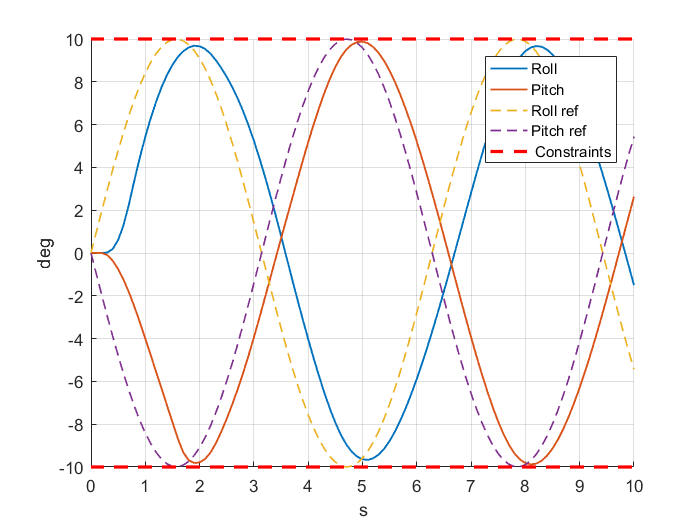
\includegraphics[width=\linewidth]{Plots_06_ReferenceTracking_Varying/01}
            \caption{Roll and Pitch}
        \end{subfigure}
        ~
        \begin{subfigure}[c]{0.3\linewidth}
            \centering
            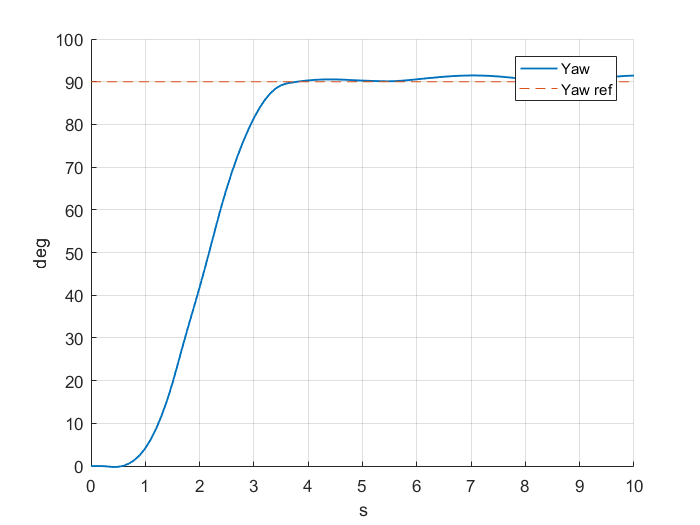
\includegraphics[width=\linewidth]{Plots_06_ReferenceTracking_Varying/02}
            \caption{Yaw}
        \end{subfigure}
        ~
        \begin{subfigure}[c]{0.3\linewidth}
            \centering
            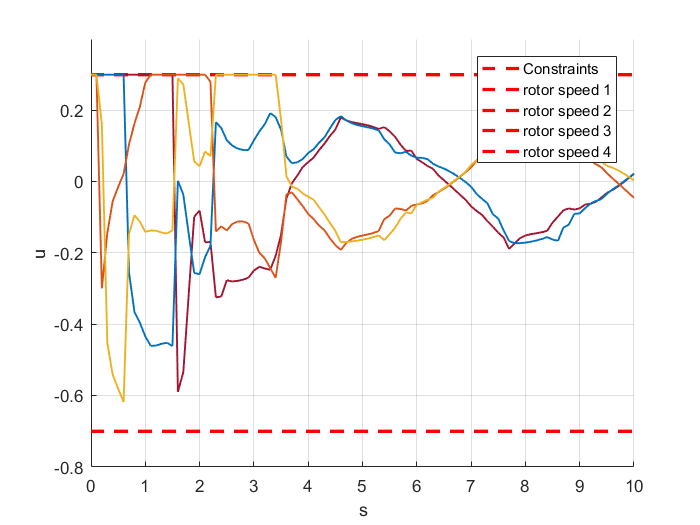
\includegraphics[width=\linewidth]{Plots_06_ReferenceTracking_Varying/03}
            \caption{Rotor Speeds}
        \end{subfigure}

        \begin{subfigure}[c]{0.3\linewidth}
            \centering
            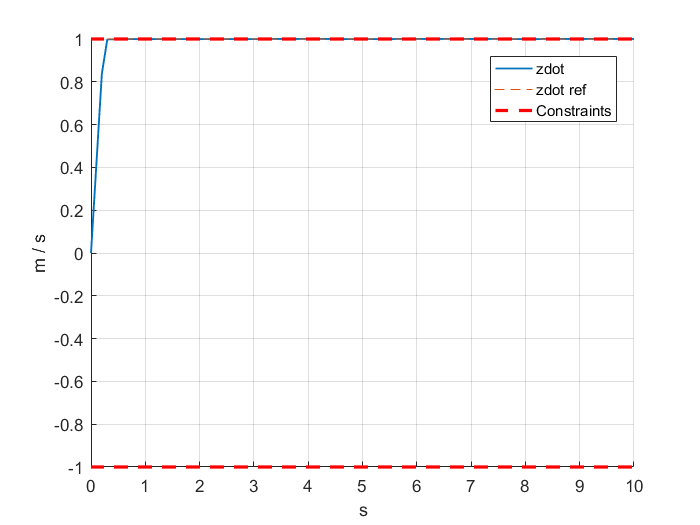
\includegraphics[width=\linewidth]{Plots_06_ReferenceTracking_Varying/04}
            \caption{zdot}
        \end{subfigure}
        ~
        \begin{subfigure}[c]{0.3\linewidth}
            \centering
            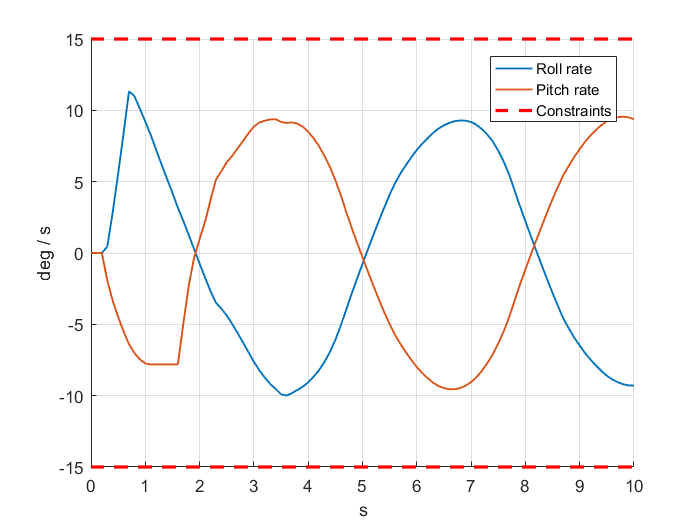
\includegraphics[width=\linewidth]{Plots_06_ReferenceTracking_Varying/05}
            \caption{Roll and Pitch rates}
        \end{subfigure}
        ~
        \begin{subfigure}[c]{0.3\linewidth}
            \centering
            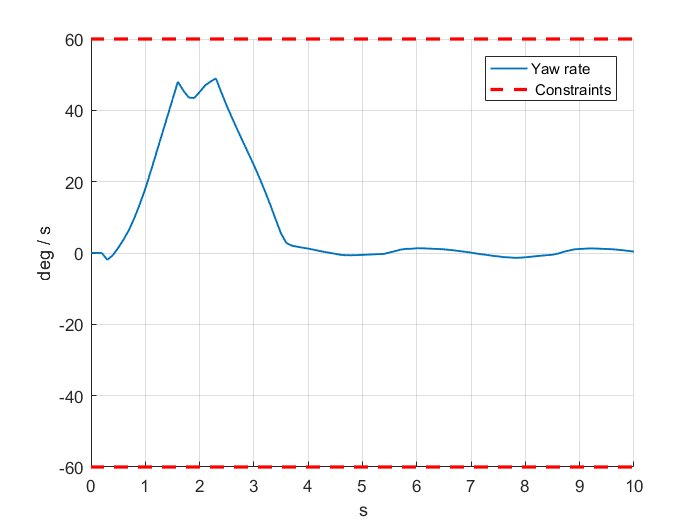
\includegraphics[width=\linewidth]{Plots_06_ReferenceTracking_Varying/06}
            \caption{Yaw rate}
        \end{subfigure}
        \caption{Response for a slowly varying reference signal with offset.}
        \label{fig:varying_reference_with_offset}
\end{figure}
\end{enumerate}

% subsection reference_tracking (end)


\subsection*{First simulation of the nonlinear model} % (fold)
\label{sub:first_simulation_of_the_nonlinear_model}

\begin{enumerate}
    \setcounter{enumi}{6}
    % 7.
    \item The response of the reference tracking of the nonlinear model can be
    seen in Figure~\ref{fig:nonlinear_reference_tracking_with_offset}.
    \begin{figure}[ht]
        \centering
        \begin{subfigure}[c]{0.3\linewidth}
            \centering
            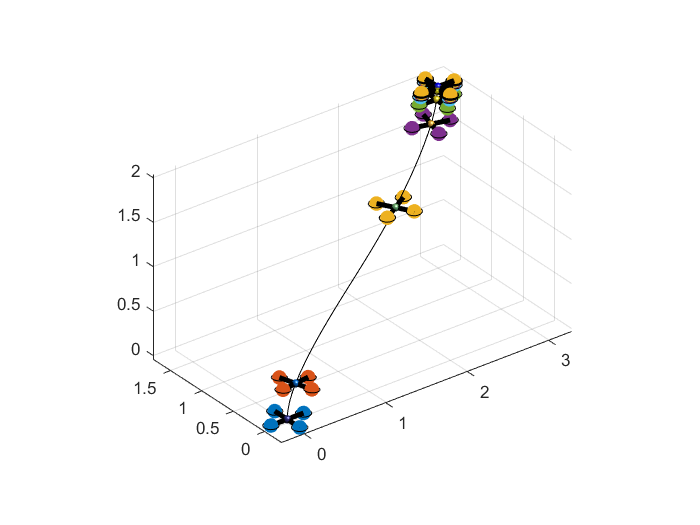
\includegraphics[width=\linewidth]{Plots_07_NonlinearModel_ReferenceTracking/01}
            \caption{Quadrotor}
        \end{subfigure}
        ~
        \begin{subfigure}[c]{0.3\linewidth}
            \centering
            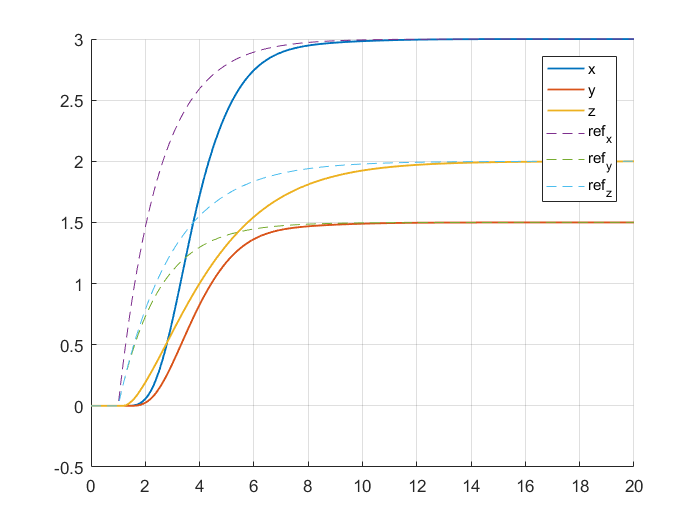
\includegraphics[width=\linewidth]{Plots_07_NonlinearModel_ReferenceTracking/02}
            \caption{x, y and z}
        \end{subfigure}
        ~
        \begin{subfigure}[c]{0.3\linewidth}
            \centering
            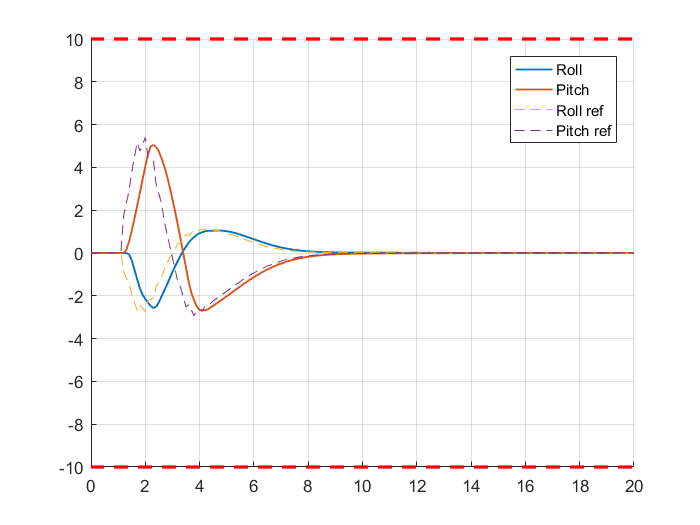
\includegraphics[width=\linewidth]{Plots_07_NonlinearModel_ReferenceTracking/03}
            \caption{Roll and Pitch}
        \end{subfigure}

        \begin{subfigure}[c]{0.3\linewidth}
            \centering
            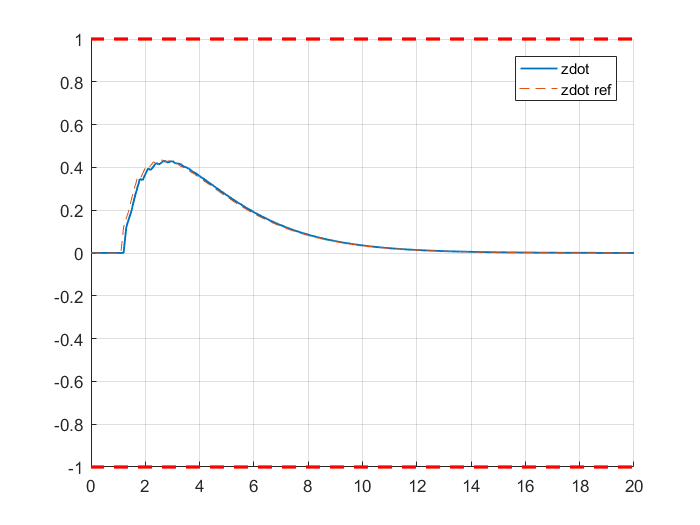
\includegraphics[width=\linewidth]{Plots_07_NonlinearModel_ReferenceTracking/04}
            \caption{zdot}
        \end{subfigure}
        ~
        \begin{subfigure}[c]{0.3\linewidth}
            \centering
            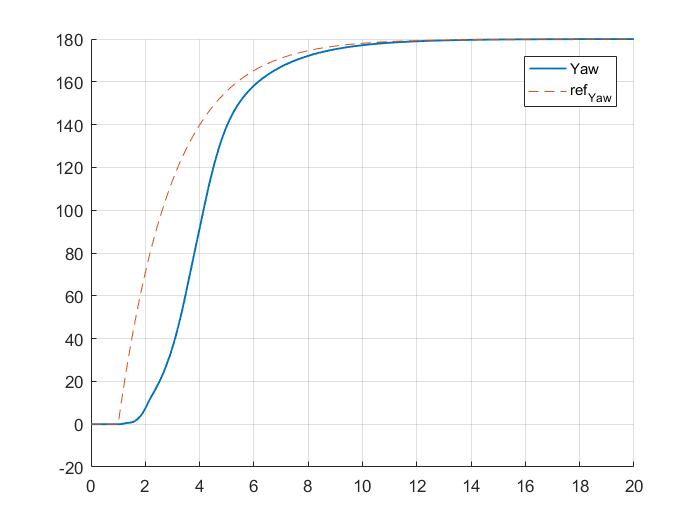
\includegraphics[width=\linewidth]{Plots_07_NonlinearModel_ReferenceTracking/05}
            \caption{Yaw}
        \end{subfigure}
        ~
        \begin{subfigure}[c]{0.3\linewidth}
            \centering
            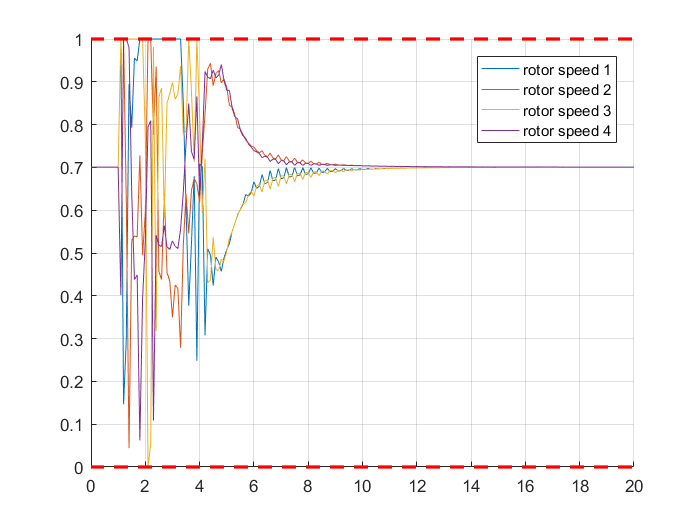
\includegraphics[width=\linewidth]{Plots_07_NonlinearModel_ReferenceTracking/06}
            \caption{Rotor Speeds}
        \end{subfigure}

        \begin{subfigure}[c]{0.3\linewidth}
            \centering
            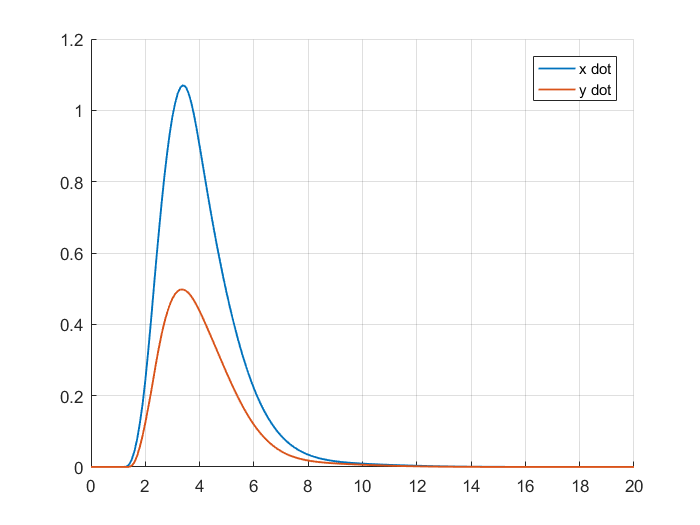
\includegraphics[width=\linewidth]{Plots_07_NonlinearModel_ReferenceTracking/07}
            \caption{xdot and ydot}
        \end{subfigure}
        ~
        \begin{subfigure}[c]{0.3\linewidth}
            \centering
            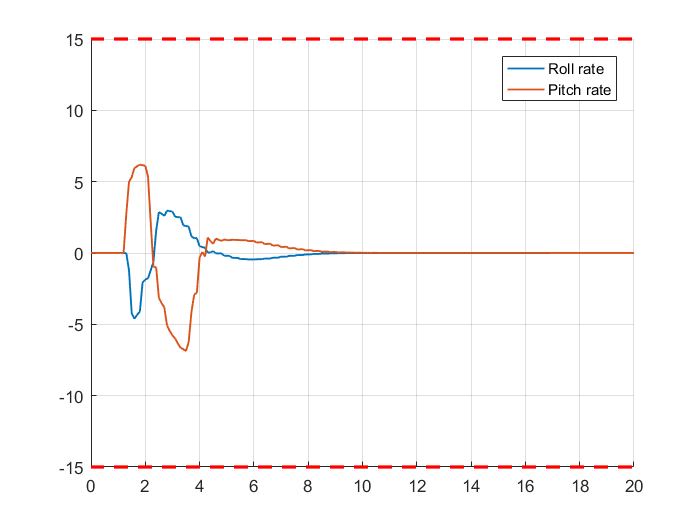
\includegraphics[width=\linewidth]{Plots_07_NonlinearModel_ReferenceTracking/08}
            \caption{Roll and Pitch rate}
        \end{subfigure}
        ~
        \begin{subfigure}[c]{0.3\linewidth}
            \centering
            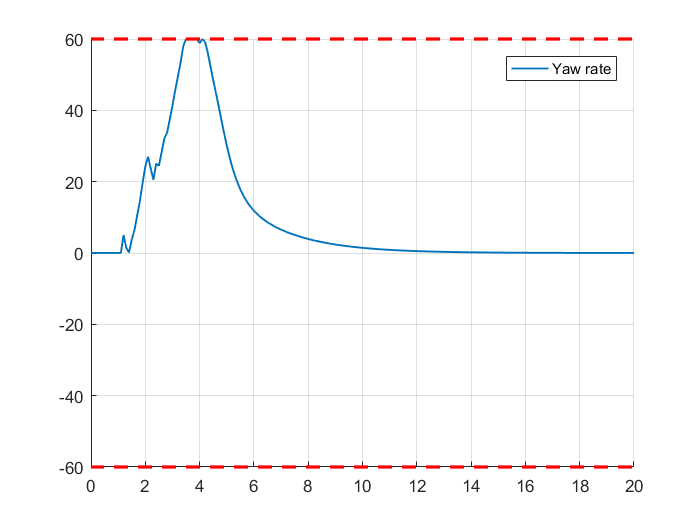
\includegraphics[width=\linewidth]{Plots_07_NonlinearModel_ReferenceTracking/09}
            \caption{Yaw rate}
        \end{subfigure}
        \caption{Reference tracking response of the nonlinear model.}
        \label{fig:nonlinear_reference_tracking_with_offset}
\end{figure}
\end{enumerate}

% subsection first_simulation_of_the_nonlinear_model (end)


\subsection*{Offset free MPC} % (fold)
\label{sub:offset_free_mpc}

\begin{enumerate}
    \setcounter{enumi}{7}
    % 8.
    \item The matrix L:
    
    Our calculation of L is based on the solution of the dual LQR-problem for the augmented system.
    
    \begin{verbatim}
    L = dlqr(A_aug',C_aug',Q_aug,R_aug)';
    \end{verbatim}
    
    For this purpose special weighting matrices $Q_{aug}$ and $R_{aug}$ were designed. Those were chosen as follows:
    
    \begin{verbatim}
    Q_aug = diag([ones(1,nx) [50 1 1 500 10 10 0.01]);
    R_aug = eye(nx);
    \end{verbatim}
    
    Reasoning for the selection of $Q_{aug}$ and $R_{aug}$:
    
    \begin{itemize}
    \item The weighting of the state-estimates were chosen relatively low since we don't need them.
    \item The weighting of the disturbance estimates were chosen slightly higher. We chose higher weighting for less noisy measurements and lower weightings for more noisy measurements thereby dampening the noise.
    \end{itemize}
    
    \begin{equation}
    L = \begin{bmatrix} 
    0.8966&0&0&0&0&0&0\\
    0&0.5808&0&0&0.0317&0&0\\
    0&0&0&0.9821&0&0&0.0307\\
    0&0.0015&0&0&0.7758&0&0\\
    0&0&0.0015&0&0&0.7758&0\\
    0&0&0&0.0001&0&0&0.3316\\
    0.7191&0&0&0&0&0&0\\
    0&0.2050&0&0&0.0017&0&0\\
    0&0&0.2050&0&0&0.0017&0\\
    0&0&0&0.9458&0&0&-0.0211\\
    0&-0.0106&0&0&0.4734&0&0\\
    0&0&-0.0106&0&0&0.4734&0\\
    0&0&0&0&0&0&0.0259\\
    \end{bmatrix}
    \end{equation}
    
	% 9.
	\item The response of the offset free tracking with a constant reference can be
    seen in Figure~\ref{fig:offset_free_tracking_with_constant}.
    \begin{figure}[ht]
        \centering
        \begin{subfigure}[c]{0.3\linewidth}
            \centering
            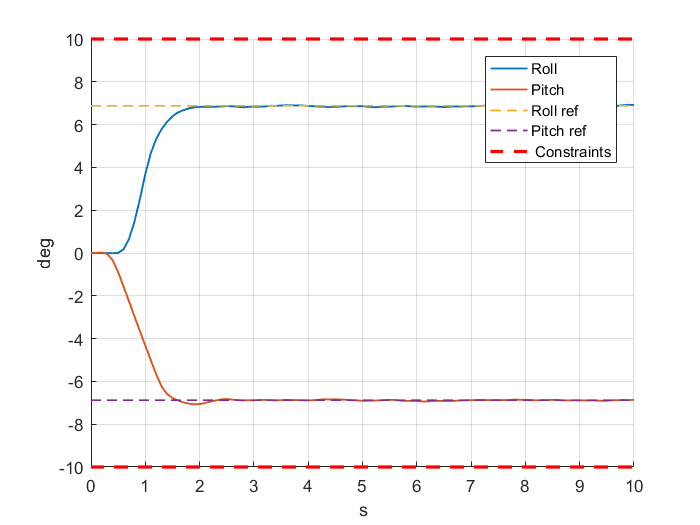
\includegraphics[width=\linewidth]{Plots_09_OffsetFreeTracking_Constant/01}
            \caption{Roll and Pitch}
        \end{subfigure}
        ~
        \begin{subfigure}[c]{0.3\linewidth}
            \centering
            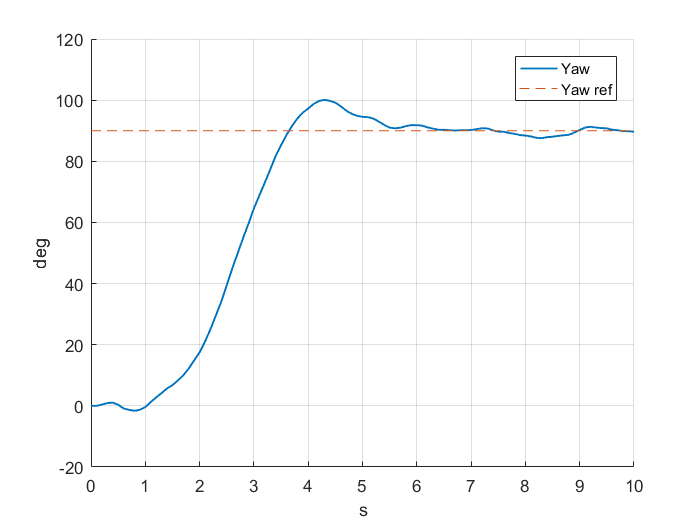
\includegraphics[width=\linewidth]{Plots_09_OffsetFreeTracking_Constant/02}
            \caption{Yaw}
        \end{subfigure}
        ~
        \begin{subfigure}[c]{0.3\linewidth}
            \centering
            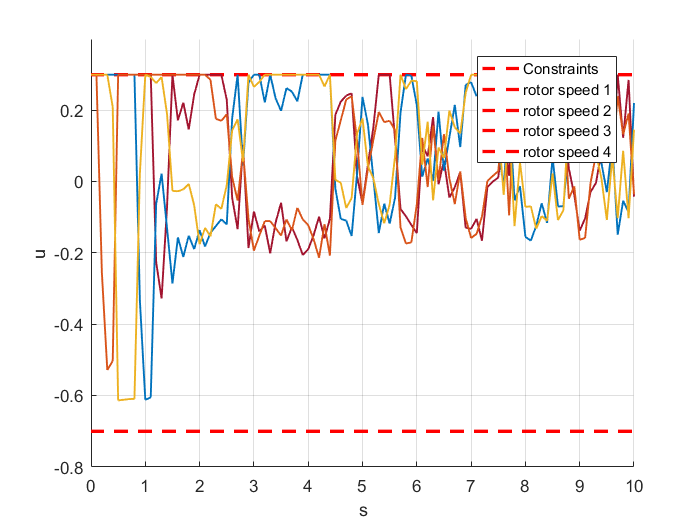
\includegraphics[width=\linewidth]{Plots_09_OffsetFreeTracking_Constant/03}
            \caption{Rotor Speeds}
        \end{subfigure}

        \begin{subfigure}[c]{0.3\linewidth}
            \centering
            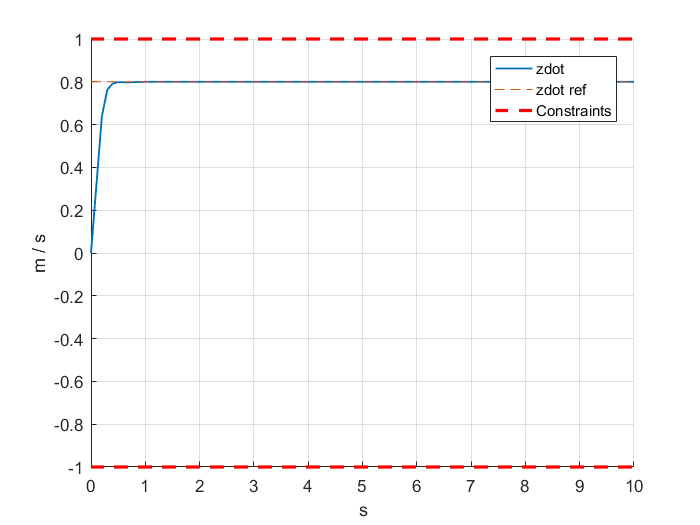
\includegraphics[width=\linewidth]{Plots_09_OffsetFreeTracking_Constant/04}
            \caption{zdot}
        \end{subfigure}
        ~
        \begin{subfigure}[c]{0.3\linewidth}
            \centering
            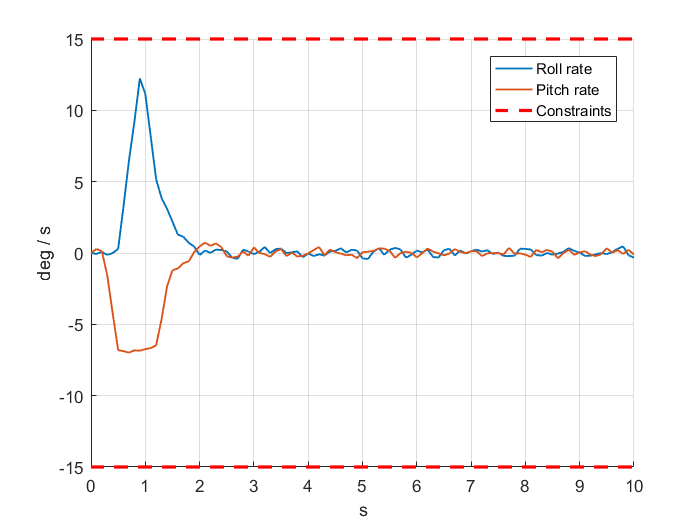
\includegraphics[width=\linewidth]{Plots_09_OffsetFreeTracking_Constant/05}
            \caption{Roll and Pitch rates}
        \end{subfigure}
        ~
        \begin{subfigure}[c]{0.3\linewidth}
            \centering
            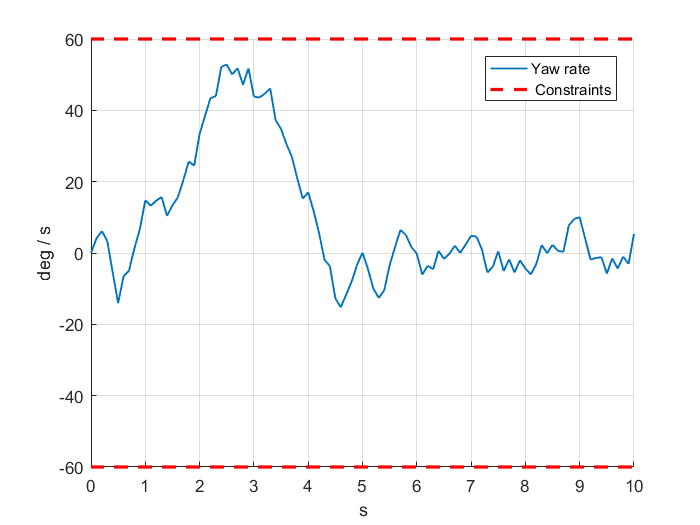
\includegraphics[width=\linewidth]{Plots_09_OffsetFreeTracking_Constant/06}
            \caption{Yaw rate}
        \end{subfigure}

        \begin{subfigure}[c]{0.3\linewidth}
            \centering
            \includegraphics[width=\linewidth]{Plots_09_OffsetFreeTracking_Constant/08}
            \caption{zdot disturbance}
        \end{subfigure}
        ~
        \begin{subfigure}[c]{0.3\linewidth}
            \centering
            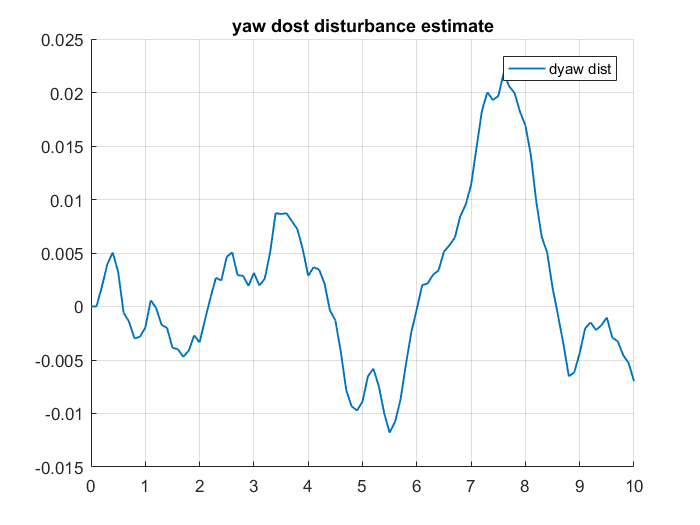
\includegraphics[width=\linewidth]{Plots_09_OffsetFreeTracking_Constant/09}
            \caption{Yawdot disturbance}
        \end{subfigure}
        ~
        \begin{subfigure}[c]{0.3\linewidth}
            \centering
            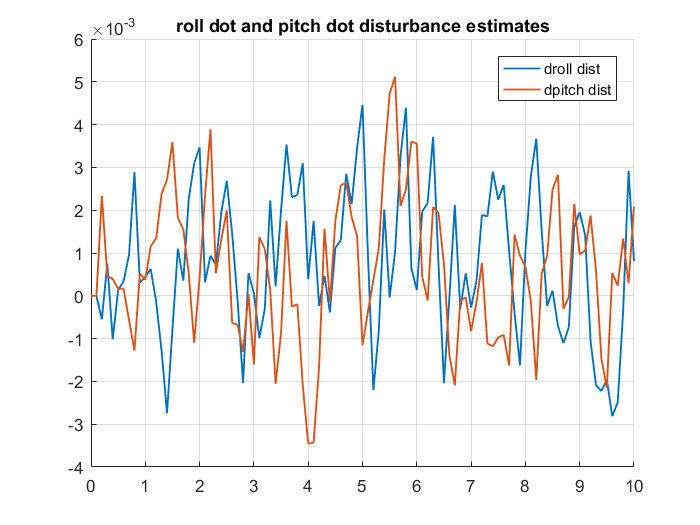
\includegraphics[width=\linewidth]{Plots_09_OffsetFreeTracking_Constant/10}
            \caption{Disturbance of $\dot{\alpha}$ and $\dot{\beta}$}
        \end{subfigure}
        \caption{Offset-free tracking with a constant reference.}
        \label{fig:offset_free_tracking_with_constant}
\end{figure}

    % 10.
    \item The response of the offset free tracking with a varying reference can be
    seen in Figure~\ref{fig:offset_free_tracking_with_varying}.
    \begin{figure}[ht]
        \centering
        \begin{subfigure}[c]{0.3\linewidth}
            \centering
            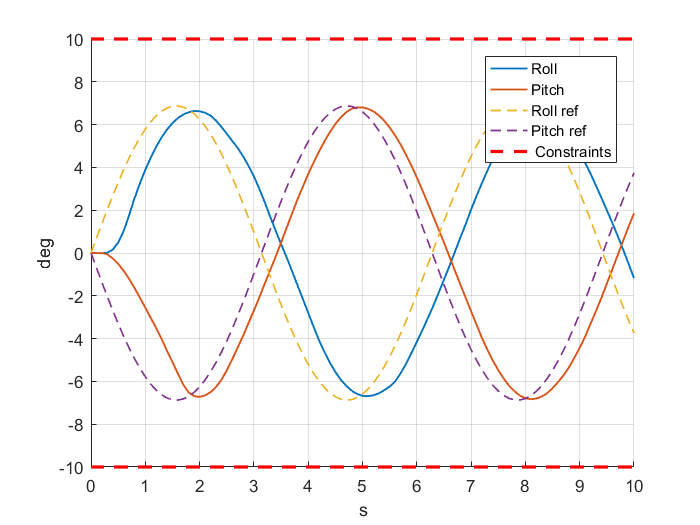
\includegraphics[width=\linewidth]{Plots_10_OffsetFreeTracking_Varying/01}
            \caption{Roll and Pitch}
        \end{subfigure}
        ~
        \begin{subfigure}[c]{0.3\linewidth}
            \centering
            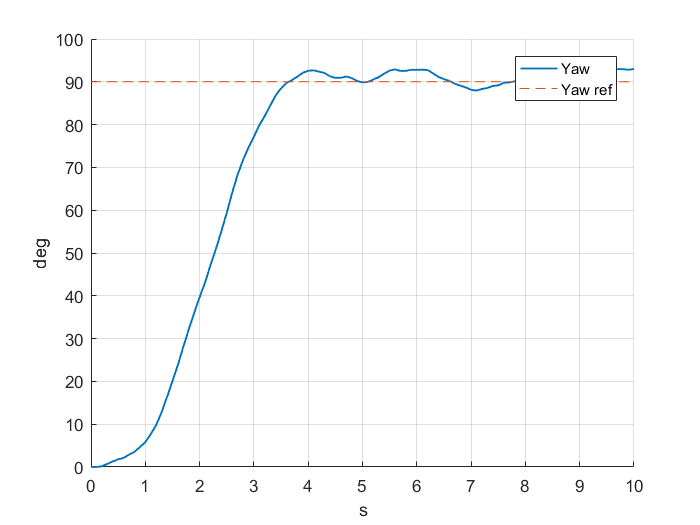
\includegraphics[width=\linewidth]{Plots_10_OffsetFreeTracking_Varying/02}
            \caption{Yaw}
        \end{subfigure}
        ~
        \begin{subfigure}[c]{0.3\linewidth}
            \centering
            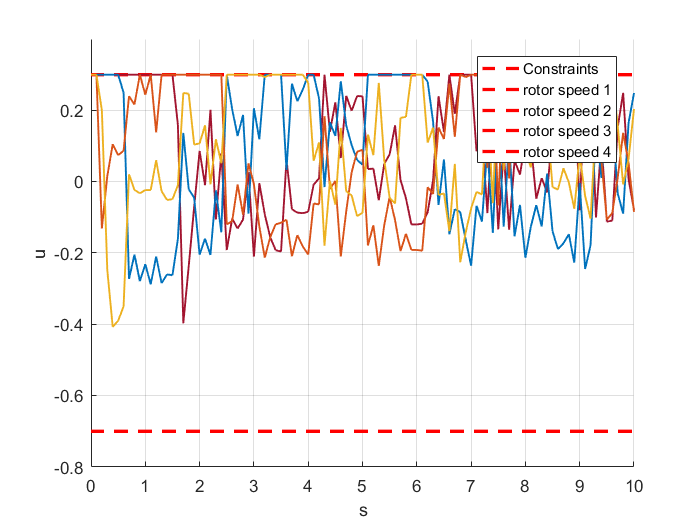
\includegraphics[width=\linewidth]{Plots_10_OffsetFreeTracking_Varying/03}
            \caption{Rotor Speeds}
        \end{subfigure}

        \begin{subfigure}[c]{0.3\linewidth}
            \centering
            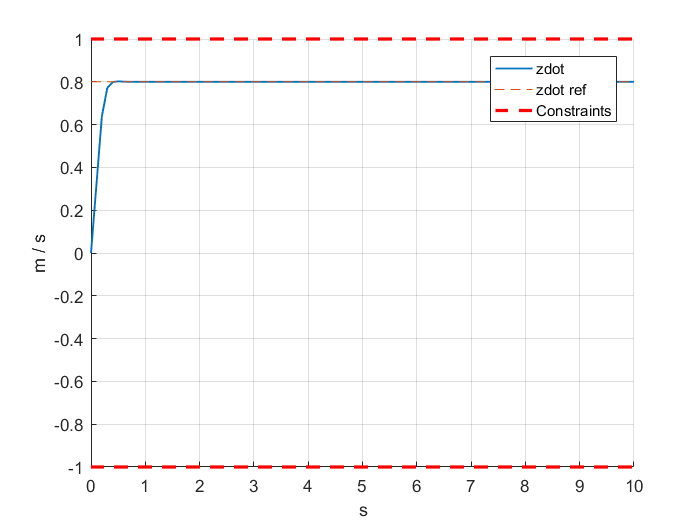
\includegraphics[width=\linewidth]{Plots_10_OffsetFreeTracking_Varying/04}
            \caption{zdot}
        \end{subfigure}
        ~
        \begin{subfigure}[c]{0.3\linewidth}
            \centering
            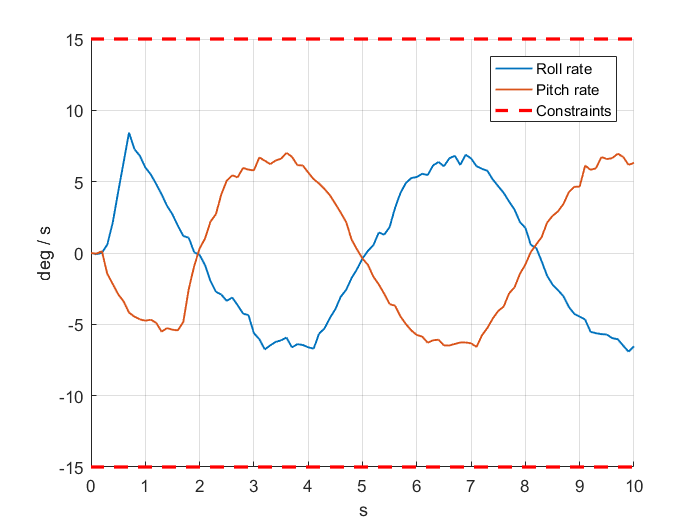
\includegraphics[width=\linewidth]{Plots_10_OffsetFreeTracking_Varying/05}
            \caption{Roll and Pitch rates}
        \end{subfigure}
        ~
        \begin{subfigure}[c]{0.3\linewidth}
            \centering
            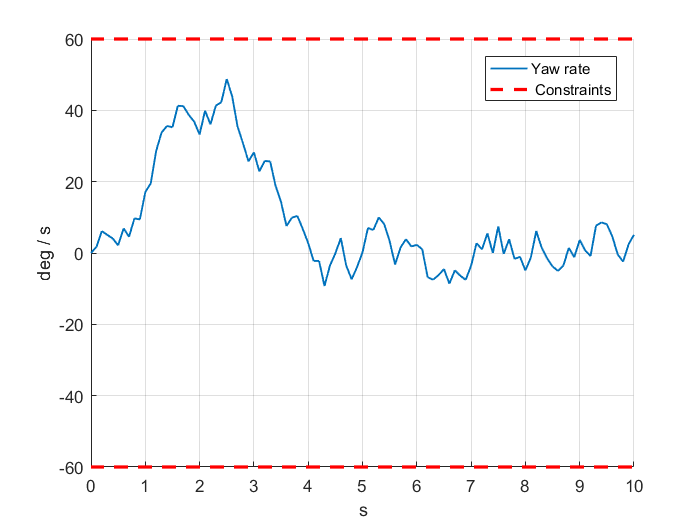
\includegraphics[width=\linewidth]{Plots_10_OffsetFreeTracking_Varying/06}
            \caption{Yaw rate}
        \end{subfigure}

        \begin{subfigure}[c]{0.3\linewidth}
            \centering
            \includegraphics[width=\linewidth]{Plots_10_OffsetFreeTracking_Varying/08}
            \caption{zdot disturbance}
        \end{subfigure}
        ~
        \begin{subfigure}[c]{0.3\linewidth}
            \centering
            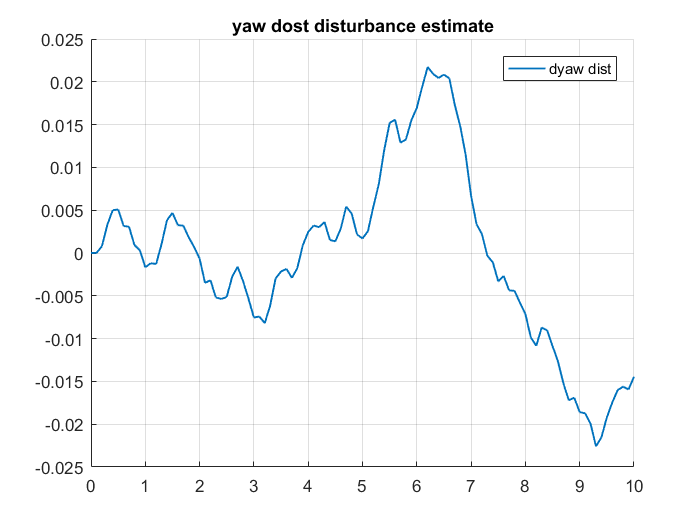
\includegraphics[width=\linewidth]{Plots_10_OffsetFreeTracking_Varying/09}
            \caption{Yawdot disturbance}
        \end{subfigure}
        ~
        \begin{subfigure}[c]{0.3\linewidth}
            \centering
            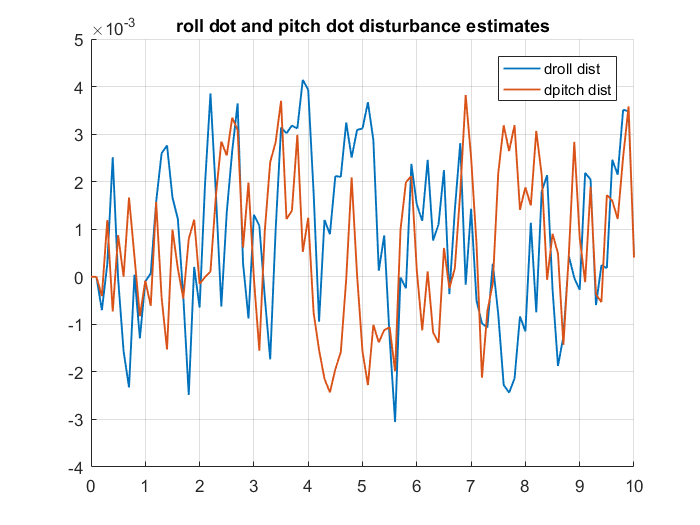
\includegraphics[width=\linewidth]{Plots_10_OffsetFreeTracking_Varying/10}
            \caption{Disturbance of $\dot{\alpha}$ and $\dot{\beta}$}
        \end{subfigure}
        \caption{Offset-free tracking with a varying reference.}
        \label{fig:offset_free_tracking_with_varying}
\end{figure}
    
\end{enumerate}

% subsection offset_free_mpc (end)


\subsection*{Simulation of the nonlinear model} % (fold)
\label{sub:simulation_of_the_nonlinear_model}

\begin{enumerate}
    \setcounter{enumi}{10}
    % 11.
    \item The response of the nonlinear model to a step signal can be
    seen in Figure~\ref{fig:nonlinear_model_step_signal}.
    \begin{figure}[ht]
        \centering
        \begin{subfigure}[c]{0.3\linewidth}
            \centering
            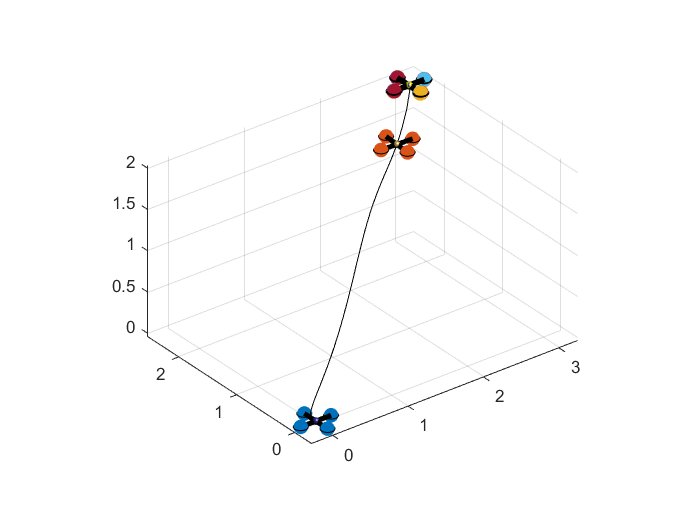
\includegraphics[width=\linewidth]{Plots_11_NonlinearModel_StepSignal/01}
            \caption{Quadrotor}
        \end{subfigure}
        ~
        \begin{subfigure}[c]{0.3\linewidth}
            \centering
            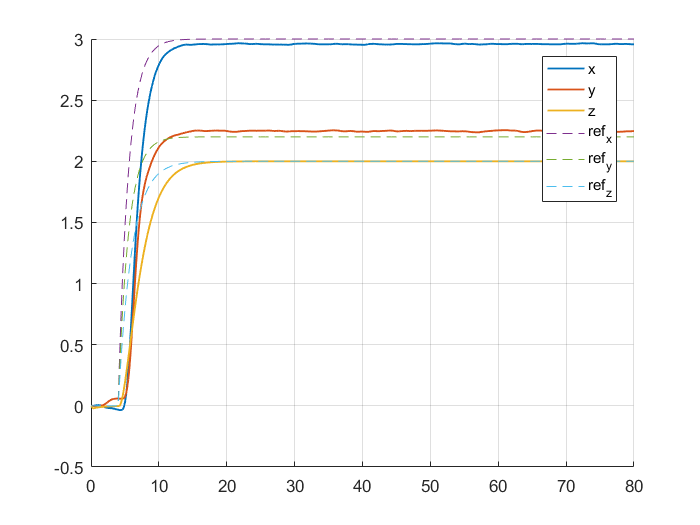
\includegraphics[width=\linewidth]{Plots_11_NonlinearModel_StepSignal/02}
            \caption{x, y and z}
        \end{subfigure}
        ~
        \begin{subfigure}[c]{0.3\linewidth}
            \centering
            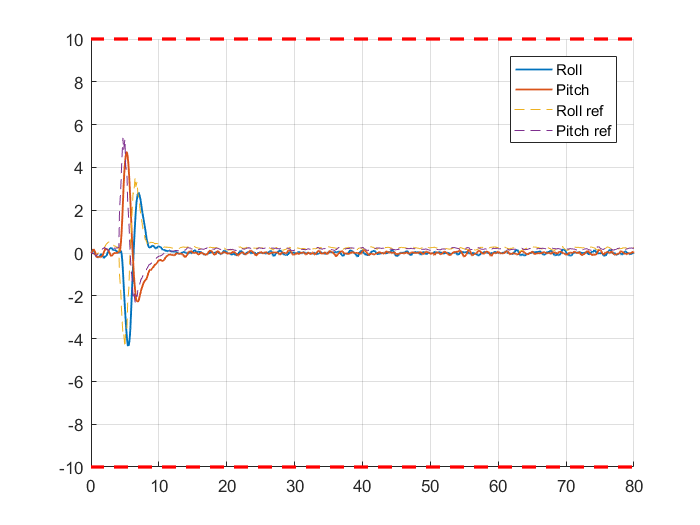
\includegraphics[width=\linewidth]{Plots_11_NonlinearModel_StepSignal/03}
            \caption{Roll and Pitch}
        \end{subfigure}
        
        \begin{subfigure}[c]{0.3\linewidth}
            \centering
            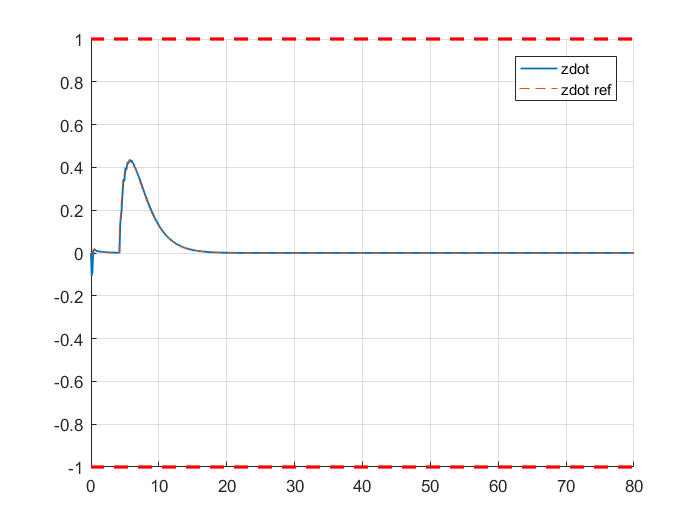
\includegraphics[width=\linewidth]{Plots_11_NonlinearModel_StepSignal/04}
            \caption{zdot}
        \end{subfigure}
        ~
        \begin{subfigure}[c]{0.3\linewidth}
            \centering
            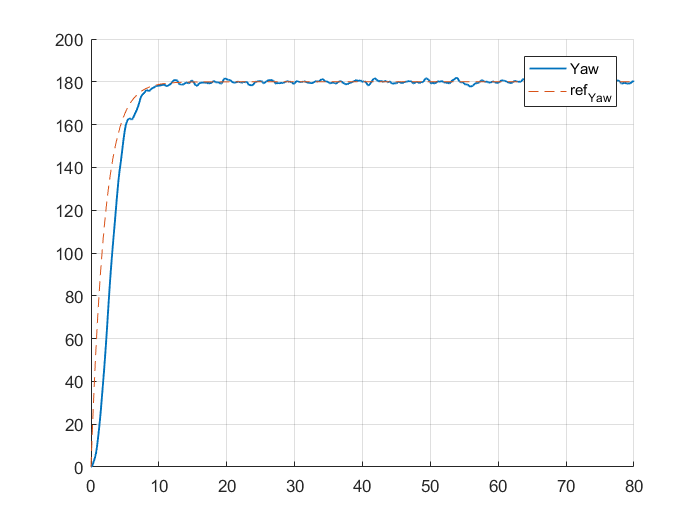
\includegraphics[width=\linewidth]{Plots_11_NonlinearModel_StepSignal/05}
            \caption{Yaw}
        \end{subfigure}
        ~
        \begin{subfigure}[c]{0.3\linewidth}
            \centering
            \includegraphics[width=\linewidth]{Plots_11_NonlinearModel_StepSignal/06}
            \caption{Rotor Speeds}
        \end{subfigure}

        \begin{subfigure}[c]{0.3\linewidth}
            \centering
            \includegraphics[width=\linewidth]{Plots_11_NonlinearModel_StepSignal/07}
            \caption{xdot and ydot}
        \end{subfigure}
        ~
        \begin{subfigure}[c]{0.3\linewidth}
            \centering
            \includegraphics[width=\linewidth]{Plots_11_NonlinearModel_StepSignal/08}
            \caption{Roll and Pitch rates}
        \end{subfigure}
        ~
        \begin{subfigure}[c]{0.3\linewidth}
            \centering
            \includegraphics[width=\linewidth]{Plots_11_NonlinearModel_StepSignal/09}
            \caption{Yaw Rate}
        \end{subfigure}
        
        \begin{subfigure}[c]{0.3\linewidth}
            \centering
            \includegraphics[width=\linewidth]{Plots_11_NonlinearModel_StepSignal/10}
            \caption{zdot disturbance}
        \end{subfigure}
        ~
        \begin{subfigure}[c]{0.3\linewidth}
            \centering
            \includegraphics[width=\linewidth]{Plots_11_NonlinearModel_StepSignal/11}
            \caption{Disturbance of $\dot{\alpha}$ and $\dot{\beta}$}
        \end{subfigure}
        
        \caption{Response of the nonlinear model with step signal.}
        \label{fig:nonlinear_model_step_signal}
\end{figure}

    % 12.
    \item The response of the nonlinear model to a hexagon signal can be
    seen in Figure~\ref{fig:nonlinear_model_hexagon_signal}.
    \begin{figure}[ht]
        \centering
        \begin{subfigure}[c]{0.3\linewidth}
            \centering
            \includegraphics[width=\linewidth]{Plots_12_NonlinearModel_Hexagon/01}
            \caption{Quadrotor}
        \end{subfigure}
        ~
        \begin{subfigure}[c]{0.3\linewidth}
            \centering
            \includegraphics[width=\linewidth]{Plots_12_NonlinearModel_Hexagon/02}
            \caption{x, y, and z}
        \end{subfigure}
        ~
        \begin{subfigure}[c]{0.3\linewidth}
            \centering
            \includegraphics[width=\linewidth]{Plots_12_NonlinearModel_Hexagon/03}
            \caption{Roll and Pitch}
        \end{subfigure}
        
        \begin{subfigure}[c]{0.3\linewidth}
            \centering
            \includegraphics[width=\linewidth]{Plots_12_NonlinearModel_Hexagon/04}
            \caption{zdot}
        \end{subfigure}
        ~
        \begin{subfigure}[c]{0.3\linewidth}
            \centering
            \includegraphics[width=\linewidth]{Plots_12_NonlinearModel_Hexagon/05}
            \caption{Yaw}
        \end{subfigure}
        ~
        \begin{subfigure}[c]{0.3\linewidth}
            \centering
            \includegraphics[width=\linewidth]{Plots_12_NonlinearModel_Hexagon/06}
            \caption{Rotor Speeds}
        \end{subfigure}

        \begin{subfigure}[c]{0.3\linewidth}
            \centering
            \includegraphics[width=\linewidth]{Plots_12_NonlinearModel_Hexagon/07}
            \caption{xdot and ydot}
        \end{subfigure}
        ~
        \begin{subfigure}[c]{0.3\linewidth}
            \centering
            \includegraphics[width=\linewidth]{Plots_12_NonlinearModel_Hexagon/08}
            \caption{Roll and Pitch rates}
        \end{subfigure}
        ~
        \begin{subfigure}[c]{0.3\linewidth}
            \centering
            \includegraphics[width=\linewidth]{Plots_12_NonlinearModel_Hexagon/09}
            \caption{Yaw rate}
        \end{subfigure}
        
        \begin{subfigure}[c]{0.3\linewidth}
            \centering
            \includegraphics[width=\linewidth]{Plots_12_NonlinearModel_Hexagon/10}
            \caption{zdot disturbance}
        \end{subfigure}
        ~
        \begin{subfigure}[c]{0.3\linewidth}
            \centering
            \includegraphics[width=\linewidth]{Plots_12_NonlinearModel_Hexagon/11}
            \caption{Disturbance of $\dot{\alpha}$ and $\dot{\beta}$}
        \end{subfigure}
        
        \caption{Nonlinear model with hexagon signal.}
        \label{fig:nonlinear_model_hexagon_signal}
\end{figure}

    % 13.
    \item The response of the nonlinear model to a lemniscate signal can be
    seen in Figure~\ref{fig:nonlinear_model_lemniscate_signal}.
    \begin{figure}[ht]
        \centering
        \begin{subfigure}[c]{0.3\linewidth}
            \centering
            \includegraphics[width=\linewidth]{Plots_13_NonlinearModel_Lemniscate/01}
            \caption{Quadrotor}
        \end{subfigure}
        ~
        \begin{subfigure}[c]{0.3\linewidth}
            \centering
            \includegraphics[width=\linewidth]{Plots_13_NonlinearModel_Lemniscate/02}
            \caption{x, y, and z}
        \end{subfigure}
        ~
        \begin{subfigure}[c]{0.3\linewidth}
            \centering
            \includegraphics[width=\linewidth]{Plots_13_NonlinearModel_Lemniscate/03}
            \caption{Roll and Pitch}
        \end{subfigure}
        
        \begin{subfigure}[c]{0.3\linewidth}
            \centering
            \includegraphics[width=\linewidth]{Plots_13_NonlinearModel_Lemniscate/04}
            \caption{zdot}
        \end{subfigure}
        ~
        \begin{subfigure}[c]{0.3\linewidth}
            \centering
            \includegraphics[width=\linewidth]{Plots_13_NonlinearModel_Lemniscate/05}
            \caption{Yaw}
        \end{subfigure}
        ~
        \begin{subfigure}[c]{0.3\linewidth}
            \centering
            \includegraphics[width=\linewidth]{Plots_13_NonlinearModel_Lemniscate/06}
            \caption{Rotor Speeds}
        \end{subfigure}

        \begin{subfigure}[c]{0.3\linewidth}
            \centering
            \includegraphics[width=\linewidth]{Plots_13_NonlinearModel_Lemniscate/07}
            \caption{xdot and ydot}
        \end{subfigure}
        ~
        \begin{subfigure}[c]{0.3\linewidth}
            \centering
            \includegraphics[width=\linewidth]{Plots_13_NonlinearModel_Lemniscate/08}
            \caption{Roll and Pitch rates}
        \end{subfigure}
        ~
        \begin{subfigure}[c]{0.3\linewidth}
            \centering
            \includegraphics[width=\linewidth]{Plots_13_NonlinearModel_Lemniscate/09}
            \caption{Yaw rate}
        \end{subfigure}
        
        \begin{subfigure}[c]{0.3\linewidth}
            \centering
            \includegraphics[width=\linewidth]{Plots_13_NonlinearModel_Lemniscate/10}
            \caption{zdot disturbance}
        \end{subfigure}
        ~
        \begin{subfigure}[c]{0.3\linewidth}
            \centering
            \includegraphics[width=\linewidth]{Plots_13_NonlinearModel_Lemniscate/11}
            \caption{Disturbance of $\dot{\alpha}$ and $\dot{\beta}$}
        \end{subfigure}
        
        \caption{Nonlinear model with lemniscate signal.}
        \label{fig:nonlinear_model_lemniscate_signal}
\end{figure}
\end{enumerate}

% subsection simulation_of_the_nonlinear_model (end)


\subsection*{Slew rate constraints} % (fold)
\label{sub:slew_rate_constraints}

\begin{enumerate}
    \setcounter{enumi}{13}
    % 14.
    \item The response of the offset-free tracking with slew rate constraints can be
    seen in Figure~\ref{fig:slew_rate}.
    \begin{figure}[ht]
        \centering
        \begin{subfigure}[c]{0.3\linewidth}
            \centering
            \includegraphics[width=\linewidth]{Plots_14_SlewRateConstraints/01}
            \caption{Roll and Pitch}
        \end{subfigure}
        ~
        \begin{subfigure}[c]{0.3\linewidth}
            \centering
            \includegraphics[width=\linewidth]{Plots_14_SlewRateConstraints/02}
            \caption{Yaw}
        \end{subfigure}
        ~
        \begin{subfigure}[c]{0.3\linewidth}
            \centering
            \includegraphics[width=\linewidth]{Plots_14_SlewRateConstraints/03}
            \caption{Rotor Speeds}
        \end{subfigure}

        \begin{subfigure}[c]{0.3\linewidth}
            \centering
            \includegraphics[width=\linewidth]{Plots_14_SlewRateConstraints/04}
            \caption{zdot}
        \end{subfigure}
        ~
        \begin{subfigure}[c]{0.3\linewidth}
            \centering
            \includegraphics[width=\linewidth]{Plots_14_SlewRateConstraints/05}
            \caption{Roll and Pitch rates}
        \end{subfigure}
        ~
        \begin{subfigure}[c]{0.3\linewidth}
            \centering
            \includegraphics[width=\linewidth]{Plots_14_SlewRateConstraints/06}
            \caption{Yaw rate}
        \end{subfigure}

        \begin{subfigure}[c]{0.3\linewidth}
            \centering
            \includegraphics[width=\linewidth]{Plots_14_SlewRateConstraints/08}
            \caption{zdot disturbance}
        \end{subfigure}
        ~
        \begin{subfigure}[c]{0.3\linewidth}
            \centering
            \includegraphics[width=\linewidth]{Plots_14_SlewRateConstraints/09}
            \caption{Yawdot disturbance}
        \end{subfigure}
        ~
        \begin{subfigure}[c]{0.3\linewidth}
            \centering
            \includegraphics[width=\linewidth]{Plots_14_SlewRateConstraints/10}
            \caption{Disturbance of $\dot{\alpha}$ and $\dot{\beta}$}
        \end{subfigure}
        \caption{Offset-free tracking with slew rate constraints.}
        \label{fig:slew_rate}
\end{figure}
\end{enumerate}

% subsection slew_rate_constraints (end)


\subsection*{Soft Constraints} % (fold)
\label{sub:soft_constraints}

\begin{enumerate}
    \setcounter{enumi}{14}
    % 15.
    \item Could no be completed due to difficulties with SimQuad.

    % 16.
    \item Could no be completed due to difficulties with SimQuad.

\end{enumerate}

% subsection soft_constraints (end)


\subsection*{FORCES Pro} % (fold)
\label{sub:forces_pro}

\begin{enumerate}
    \setcounter{enumi}{16}
    % 17.
    \item
\end{enumerate}

% subsection forces_pro (end)

\end{document}
